\documentclass[twocolumn, 11pt]{article}
\usepackage{amsmath, amssymb, amsthm, mathtools, bm, moresize}
\usepackage{euler}

\usepackage{graphicx, epsdice, xcolor, listings, float, wrapfig, caption}
\usepackage[top=1.2in, bottom=1.2in, left=0.6in, right=0.6in]{geometry}

\usepackage{etoolbox}
\patchcmd{\thebibliography}{\section*{\refname}}{}{}{}

\newcommand{\EE}{\mathbb{E}}
\newcommand{\PP}{\mathbb{P}}
\newcommand{\RR}{\mathbb{R}}
%
\newcommand{\Dd}{\mathcal{D}}
\newcommand{\Ee}{\mathcal{E}}
\newcommand{\Ff}{\mathcal{F}}
\newcommand{\Gg}{\mathcal{G}}
\newcommand{\Hh}{\mathcal{H}}
\newcommand{\Ii}{\mathcal{I}}
\newcommand{\Kk}{\mathcal{K}}
\newcommand{\Ll}{\mathcal{L}}
\newcommand{\Ss}{\mathcal{S}}
\newcommand{\Tt}{\mathcal{T}}
\newcommand{\Uu}{\mathcal{U}}
\newcommand{\Vv}{\mathcal{V}}
\newcommand{\Xx}{\mathcal{X}}
\newcommand{\Yy}{\mathcal{Y}}

\newcommand{\Ein} {\text{trn}_{\Ss}} %{\Ee_{\text{in},\Uu}}
\newcommand{\Einb} {\text{trn}_{\check\Ss}} %{\Ee_{\text{in},\Uu}}
\newcommand{\Einc} {\text{trn}_{\Ss\sqcup \check\Ss}} %{\Ee_{\text{in},\Uu}}
\newcommand{\Egap}{\text{gap}_{\Ss}}
\newcommand{\Eout}{\text{tst}} %{\Ee_{\text{out}}}

\newtheorem*{qst}{Question}
\newtheorem*{thm}{Theorem}
\newtheorem*{lem}{Lemma}
\theoremstyle{definition}
\newtheorem*{dfn}{Definition}

\definecolor{mblu}{rgb}{0.05, 0.40, 0.70}
\newcommand{\msec}[1]{\subsection*{\color{mblu}\textsf{#1}}}

\begin{document}

    \twocolumn[
        \begin{@twocolumnfalse}
            \begin{tabular}{p{0.06\linewidth}p{0.9\linewidth}}
                &
                \begin{flushleft}  \Huge \color{mblu} \bf\textsf{WHAT IS...}    \vspace{0.1cm}\\\hrule  \end{flushleft} \vspace{-1.0\baselineskip}
                \begin{flushright} \HUGE \color{mblu} \bf the VC-Dimension?    \end{flushright} \vspace{-1.0\baselineskip}
                \begin{flushright} \Large             \it Samuel C.\ Tenka      \end{flushright}
            \end{tabular}
        \end{@twocolumnfalse}
    ]

    \msec{Wetzel's Cake Problem}

        Combinatorists and bakers alike know the sequence $1, 2, 4, 8, 16,
        \cdots$ by heart.  It continues, of course, with $31$, for its $n$th
        element $c(n)$ counts the pieces obtained from a disk-shaped cake by
        cutting along all ${n\choose 2}$ lines determined by $n$ generic points
        on the cake's boundary.

        \begin{figure}[H]
            \centering
            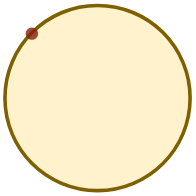
\includegraphics[height=2.3cm]{cake-1}
            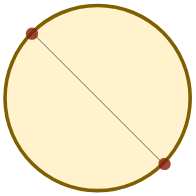
\includegraphics[height=2.3cm]{cake-2}
            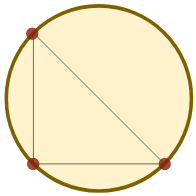
\includegraphics[height=2.3cm]{cake-3}
            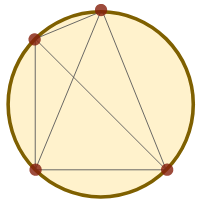
\includegraphics[height=2.3cm]{cake-4}
            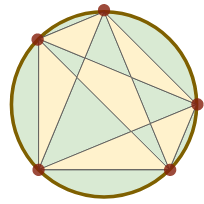
\includegraphics[height=2.3cm]{cake-5-col}
            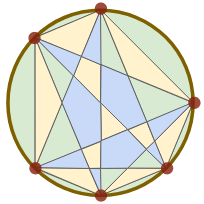
\includegraphics[height=2.3cm]{cake-6-col}
            \caption{{
                Cakes for $n=1,\cdots,6$.
                The $n=4$ cake (bottom left) has $c(4)=8$ pieces.
                Using colors to ease counting,
                we see that $c(6)$ is odd: the pieces besides the
                central yellow triangle partition into sets of six.
            }}
        \end{figure}

        In fact, $c(n)$ is a polynomial \cite{wetzel}.  We may compute $c(n)$
        by regarding a sliced cake as a planar graph, noting that two cuts (and
        hence four boundary vertices) determine each interior vertex, and
        applying Euler's formula.  One finds that $c(n)$ is ${n-1 \choose
        0}+\cdots+{n-1\choose 4}$, which explains why $c(n)$ initially
        coincides with $2^{n-1}$.

        Patterns do not always generalize.  But then how is learning from 
        data
        possible at all? 
        %
        That is, if from a collection $\Hh$ of possible patterns we find
        some $f\in \Hh$ that matches or performs well on $N$ observed data
        points, when should we expect that $f$ matches unseen data?  This
        question motivates machine learning's theory and guides its practice.

    \msec{Learning and Generalization}
        Let us precisely frame a simple case of the problem.
        Say that $\Xx$ is a space of images, $\{\pm 1\} =
        \{\text{Cow}, \text{Dog}\}$ is a set of labels, and we seek a
        classifier $f: \Xx\to\{\pm 1\}$ that accords with nature.  More
        precisely, we model nature as a probability distribution $\Dd$ over the
        space $\{\pm 1\}\times\Xx$ of labeled images and we fix a set $\Hh
        \subseteq \{\pm 1\}^\Xx$ of candidate classifiers.  With $\Ss \sim
        \Dd^N$ denoting $N$ samples drawn i.i.d.\ from $\Dd$, the
        \textbf{training error} of $f\in \Hh$ averages over the empirical
        distribution $\Ss$:
        $$
            \Ein(f) = \PP_{(y,x)\sim \Ss}[f(x)\neq y] 
        $$
        and the \textbf{testing error} averages over $\Dd$:
        $$
            \Eout(f) = \PP_{(y,x)\sim \Dd}[f(x)\neq y] 
        $$

        To learn well is to map an $\Ss$ to an $f$ with low testing error.  We
        call a map $\Ll: (\{\pm 1\}\times\Xx)^N \to \Hh$ a \textbf{learning
        rule}.  $\Ll$ might be defined by an approximate minimization of the
        training error over $\Hh$.  Then the testing error decomposes into the
        failures
        of $\Ein$ to estimate $\Eout$ (generalization),
        of $\Ll$ to minimize $\Ein$ (optimization), and 
        of $\Hh$ to contain nature's truth (approximation): 
        \newcommand{\minf}[1]{{\inf}_{\Hh}}%\inf_{f^\prime\in#1}}
        \begin{align*}
            \Eout(\Ll(\Ss)) 
            =~&\Eout(\Ll(\Ss))           &-~&           \Ein(\Ll(\Ss))& \text{gener.} \\
            +~&\Ein(\Ll(\Ss))            &-~& \minf{\Hh}(\Ein(f))& \text{optim.} \\
            +~&\minf{\Hh}(\Ein(f))  &  &                         & \text{approx.}  
        \end{align*}
        
        Focusing on the top term, we wonder when we may bound the
        \textbf{generalization gap} 
        $$
            \Egap(\Ll) = \Eout(\Ll(\Ss)) - \Ein(\Ll(\Ss)) 
        $$
        When $\Ll(\Ss)$ and $\Ss$ are independent (e.g.\ if $|\Hh|=1$),
        $\Ein(\Ll(\Ss))$ is an unbiased estimate of $\Eout(\Ll(\Ss))$, so the
        Weak Law controls $\Egap$.  However, to reduce the approximation error
        we typically choose $|\Hh|$ large; can we bound the gap in
        this case, too?
        %
        We will use the techniques of concentration and symmetrization to show
        that the answer is YES for ``finite-dimensional'' $\Hh$.

    \msec{Concentration}

        \begin{lem}[Chernoff]
            The fraction of heads among $N$ i.i.d.\ flips of a biased coin
            exceeds its mean $p$ by $g$ with chance at most 
            $\exp(-Ng^2)$, for $0 \leq p < p+g \leq 1$.
        \end{lem}

        \begin{figure}[H]
            \centering
            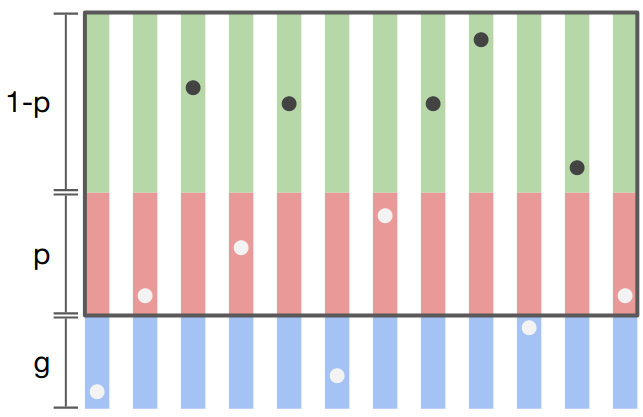
\includegraphics[height=4cm, clip]{chernoff}
            \caption{{
                We uniformly at random sample points on $N$
                sticks, each with three parts: \textbf{green}
                with length $1-p$, \textbf{red} with length $p$, and
                \textbf{blue} with length $g$.  We call non-blue points
                \textbf{boxed} and non-green points \textbf{hollow}.
            }}
            \label{fig:chernoff}
        \end{figure}

        \begin{proof} \renewcommand{\qedsymbol}{}
            Let our coin flips arise from sampling points on sticks
            (Figure \ref{fig:chernoff}), where green means tails, red
            means heads, and we condition on the event that blues do not occur.
            %
            To show that less than $(p+g)N = p^\prime N$ flips are
            heads is to show --- given that all points are \textbf{boxed} ---
            that less than $p^\prime N$ points are red. 
            %
            For any $M$:
            {%\small 
            \begin{align*}
                    & ~ \PP[\text{$M$ are red $\mid$ all are boxed}] \\
            %      = & ~ \PP[\text{$M$ are red and all are boxed}] ~/~ \PP[\text{all are boxed}]  \\
                  = & ~ \frac{\PP[\text{all hollows are red $\mid$ $M$ hollow}] \cdot \PP[\text{$M$ are hollow}]}{\PP[\text{all are boxed}] } \\
                  = & ~ (1 - g/p^\prime)^{M} \cdot (1+g)^{N} \cdot \PP[\text{$M$ are hollow}]
            \end{align*}
            }%
            We sum over $M\geq p^\prime N$, bound $\PP[\cdots p^\prime N \cdots] \leq 1$,
            then invoke $(x \mapsto x^{p^\prime})$'s concavity and
            $\exp$'s convexity:
            \begin{align*}
                &~\PP[\text{at least $p^\prime N$ are red $\mid$ all are boxed}]
                \\ \leq
                &~(1 - g/p^\prime)^{p^\prime N} \cdot (1+g)^{N} \cdot \PP[\text{at least $p^\prime N$ are hollow}]
                \\ \leq
                &~(1 - g)^N \cdot (1 + g)^{N}
                \leq
                (1 - g^2)^N
                \leq
                \exp(- Ng^2)
                ~~~~~\square
            \end{align*}
        \end{proof}

        The Chernoff bound gives us the control over tails we would expect from the
        Central Limit Theorem, but for finite instead of asymptotically large
        $N$.  In particular, when we learn from much but finite data, the
        training error will \textbf{concentrate} near the testing sample error.

        Indeed, for any $f\in \Hh$, $\Ein(f)$ is the average of $N$ independent 
        Bernoullis of mean $\Eout(f)$.  So for finite $\Hh$, the gap is
        probably small:
        \begin{align*}
            &~\PP_{\Ss\sim \Dd^N}[\Egap(\Ll) \geq g] \\
            \leq 
            &~\sum_{f\in \Hh} \PP_{\Ss\sim \Dd^N}[\Eout(f) \geq \Ein(f) + g] \\
            \leq
            &~|\Hh| \cdot \exp(-Ng^2)
        \end{align*}

        For example, if $\Hh$ is parameterized by $P$ numbers, each represented
        on a computer by $32$ bits, then $|\Hh|\leq 2^{32 P}$ and, with
        probability $1-\delta$, the gap is less than
        $$
            \sqrt{(\log(1/\delta) + 32 P)/N}
        $$
        This bound's sensitivity to the description length $32 P$ may seem
        artificial.  Indeed, the $\Hh$s used in practice --- for instance,
        linear models or neural networks --- depend smoothly on their
        parameters, so the parameters' least significant bits barely affect 
        the classifier.  In other words, $\Hh$'s cardinality is not an apt
        measure of its size.  The VC-dimension measures $\Hh$ more subtly.

    \msec{Symmetrization}

        Though $\Hh$ may be infinite, the restriction $\Hh_S = \{f|_S : f
        \in \Hh\}$ is finite for finite $S$.  If we train and test on 
        finitely many points total, we may treat $\Hh$ as finite.  Thus, let
        us estimate $\Eout(f)$, an expectation over all of $\Dd$, by
        $\Einb(f)$, an expectation over fresh samples $\check\Ss\sim \Dd^N$
        independent of the $\Ss$ from which we learn.  

        To show that $\Ein + g \geq \Eout$ when evaluated at $\Ll(\Ss)$, we
        simply show that $\Ein + g/2 \geq \Einb$ and that $\Einb +
        g/2 \geq \Eout$.  The former usually holds, since
        $|\Hh_{\Ss\sqcup\check\Ss}|$ is finite; the latter usually holds, since
        $\Ss$ and $\check\Ss$ are independent.  Quantifying with Chernoff, one
        finds that $\Egap(\Ll)$ exceeds $g$ (provided $g\geq 2/\sqrt{N}$) with
        chance at most
        \begin{align*}
            \max_{|\Ss|=|\check\Ss|=N}
            |\Hh_{\Ss\sqcup\check\Ss}| ~\cdot~ 2 \exp(-Ng^2/16)
        \end{align*}
        Thus we may control the gap by bounding $H(n) \coloneqq \max_{|S|=n}
        |\Hh_S|$.  We have achieved this reduction by putting the training and
        testing data on equal footing, hence the name \textbf{symmetrization}
        \cite{roman}.

        To progress, we bound $H(n)$.  It is clear that $H(n) \leq 2^n$.
        In fact, when this bound is loose, it is very loose:
        \begin{lem}[Sauer and Shelah]
            Unless $H(n) = 2^n$ for all $n$, $H(n)$ is bounded by a polynomial.
        \end{lem}

            \definecolor{moor}{rgb}{0.85,0.1 ,0.1 }
            \definecolor{moog}{rgb}{0.1 ,0.75,0.1 }
            \definecolor{moob}{rgb}{0.2 ,0.4 ,1.0 }
            \newcommand{\rR}[1]{{\color{moor}#1}}
            \newcommand{\gG}[1]{{\color{moog}#1}}
            \newcommand{\bB}[1]{{\color{moob}#1}}
            \newcommand{\mE}{\texttt{$\square$}}
            \newcommand{\mD}{\texttt{$\blacksquare$}}
            \newcommand{\mA}{\texttt{$\bm{+}$}}
            \newcommand{\mM}{\texttt{$\bm{-}$}}


        \begin{proof}
            Consider $\Hh_S$ for $|S|=n$.  Ordering $S$, let us write each
            $f\in \Hh_S$ as a string of plus ($+$) and minus ($-$) signs.  We
            will count these strings by translating them from the alphabet
            $\{+,-\}$ to the alphabet $\{\blacksquare,\square\}$.
            %
            Intuitively, $\blacksquare$ represents ``surprisingly $+$''.  More
            precisely, we work from left to right; whenever two (partially
            translated) strings differ \textbf{only} in their leftmost
            untranslated coordinate we overwrite the $+$ in that coordinate
            with $\blacksquare$.  Otherwise, we overwrite with $\square$.
            See Figure \ref{fig:sauer}.

            \begin{figure}[H]
                \centering
                \resizebox{\columnwidth}{!}{
                    \begin{tabular}{ccccccccc}
                           \mA \mM \mM \mM  &       &  \mE \gG\mM \mM \mM  &       &  \mE \mE \rR\mM \mM  &       &  \mE \mE \mE \rR\mM  &       &  \mE \mE \mE \mE  \\
                           \mM \mA \mM \mM  &       &  \mE \gG\mA \mM \mM  &       &  \mE \mD    \mM \mM  &       &  \mE \mD \mE \bB\mM  &       &  \mE \mD \mE \mE  \\
                           \mM \mM \mA \mM  &       &  \mE    \mM \mA \mM  &       &  \mE \mE \rR\mA \mM  &       &  \mE \mE \mD \gG\mM  &       &  \mE \mE \mD \mE  \\
                           \mM \mM \mM \mA  & $\to$ &  \mE    \mM \mM \mA  & $\to$ &  \mE \mE \gG\mM \mA  & $\to$ &  \mE \mE \mE \rR\mA  & $\to$ &  \mE \mE \mE \mD  \\
                           \mM \mM \mA \mA  &       &  \mE \bB\mM \mA \mA  &       &  \mE \mE \gG\mA \mA  &       &  \mE \mE \mD \gG\mA  &       &  \mE \mE \mD \mD  \\
                        \rR\mM \mA \mA \mA  &       &  \mE \bB\mA \mA \mA  &       &  \mE \mD    \mA \mA  &       &  \mE \mD \mE \bB\mA  &       &  \mE \mD \mE \mD  \\
                        \rR\mA \mA \mA \mA  &       &  \mD    \mA \mA \mA  &       &  \mD \mE    \mA \mA  &       &  \mD \mE \mE    \mA  &       &  \mD \mE \mE \mE
                    \end{tabular}
                }
                \caption{
                    Translating elements of $H_S$ (left) to strings of choice
                    points (right).  Each row corresponds to one of $7$ classifiers
                    and each column corresponds to one of $4$ data points.
                    %
                    We color pairs of strings that differ in-and-only-in their
                    leftmost untranslated coordinate.
                }
                \label{fig:sauer}
            \end{figure}

            Each step of translation keeps distinct strings distinct.
            %
            Moreover, whenever some $k$ indices $T\subseteq S$ of a translated
            string are $\blacksquare$s, $|\Hh_T| = 2^k$.  This is because
            $\blacksquare$s mark choice points where the classifiers attain
            both $+$ and $-$.
            %
            Now, \textbf{either} $H(n)=2^n$ for all $n$ \textbf{or} there is a
            greatest $k$ for which $H(k) = 2^k$.  In the latter case, no
            translated string may have more than $k$ $\blacksquare$s.  So
            $\Hh_S$ contains no more strings than there are subsets in $S$ of
            size $\leq k$.  In turn, we may encode each nonempty subset as the
            image of a function with a size-$k$ domain:
            $$
                H(n)
                \leq 
                {n\choose 0} + \cdots + {n\choose k}
                \leq 
                n^k + 1
            $$
            As with Wetzel's Cake, what might have grown like $2^n$ grows only
            polynomially.
        \end{proof}
    
        Since $\Hh_S$ grows no faster than the volume of a
        $k$-dimensional solid of diameter $|S|$, we call $k$ a dimension.
        \begin{dfn}
            The \textbf{Vapnik-Chervonenkis dimension} $\text{dim}(\Hh)$
            of $\Hh \subseteq \{\pm 1\}^\Xx$
            is the supremal $k$ for which $H(k) \coloneqq
            \max_{|S|=k} |\Hh_S| = 2^k$.  
        \end{dfn}

        Then $\Egap(\Ll)$ exceeds $g$ with chance at most
        \begin{align*}
            &(\text{polynomial in $N$ of degree $\text{dim}(\Hh)$}) ~\cdot~ \\
            &(\text{exponential decay in $Ng^2$})
        \end{align*}
        %\begin{align*}
        %    \label{eqn:vc}
        %    (2N+2)^{\text{dim}(\Hh)} ~\cdot~ 2 \exp(-Ng^2/16)
        %\end{align*}
        When $N\gg \text{dim}(\Hh) \log(N)$, the gap is probably small and
        generalizing from data is possible.

        For example, if $\Xx$ is a $d$-dimensional real vector space
        %$\Xx^*$ is its dual,
        and $\Hh$ is a set of ``linear classifiers''
        $$
            \Hh \subseteq \{
                \text{sign} \circ \theta
                :
                \theta \in \Xx^*
            \}
        $$
        then $\text{dim}(\Hh)$ is at most $d$,
        because any $d+1$ points $x_0, x_1,\cdots x_d \in \Xx$ engage in
        a linear relation
        $
            \sum_{i\in I} c_i x_i
            =
            \sum_{j\in J} c_j x_j
        $
        with each $c$ positive, so no $f\in \Hh$ classifies every $x_i$ as $+$
        and every $x_j$ as $-$.  A learned linear classifier will hence
        generalize when $N \gg d \log(N)$.



    \msec{Statistical Learning Theory}

        We've seen that finite VC-dimension implies that learning will
        generalize.  A converse alse holds:
        %The VC theorem, whose ``only if'' direction we've sketched,
        %summarizes the VC-dimension's role in learning theory:
        \begin{thm}[Vapnik and Chervonenkis]
            The VC-dimension of $\Hh$ is finite if and only if for all
            %data
            distributions $\Dd$, learning rules $\Ll$, and gap bounds $g>0$, the
            chance that $\Egap(\Ll)$ exceeds $g$ tends to $0$ as
            %$N=|\Ss|$ grows.  
            $N$ grows.  
        \end{thm}

        %

        The VC theorem is but one result in \textbf{statistical
        learning theory}, which abounds with variations on
        the theme that $\Egap \leq \sqrt{\log(|\Hh|/\delta)/N}$.
        %
        For instance, viewing $\log(|\Hh|)$ as the maximum entropy of
        $\Ll(\Ss) \in \Hh$, one may seek improvements given
        information-theoretic hypotheses.  Recent progress
        \cite{abbe} uses the \emph{mutual information} between $\Ss$ and
        $\Ll(\Ss)$.
        %
        Or, absent prior knowledge of $\Dd$, one may seek post hoc bounds by
        estimating properties of $\Dd$ from $\Ss$.  For example, \emph{margin
        bounds} detect when $\Dd$'s two classes are geometrically
        well-separated and hence generalization is probable \cite{mohri}.

        %\emph{Rademacher complexity}

        Other work specifically analyzes deep neural networks (nets).  The VC
        bound is
        empirically very
        loose for nets: though nets
        %seem to
        have nearly exponential $H(n)$ for typical data sets
        \cite{bengio}, they achieve state-of-the-art testing errors
        on many real-world tasks \cite{hinton}.
        %A large $H(n)$ means that nets are flexible enough to fit arbitrary
        %data.
        A large $H(n)$
        allows nets to model complex patterns yet --- in a phenomenon invisible
        to VC theory --- seems not to hinder generalization.
        %
        Thus, the mystery of modern learning: with deep neural
        networks, may we continually halve our cake and eat it, too?

    \msec{References}
        We thank A.\ Ozga and J.\ Trate for testing this
        exposition in a high school class.
        %
        The use of three-segment sticks and $\{\blacksquare,
        \square\}$-encoding to present the VC bound in elementary terms is, to
        our knowledge, new.
        %
        For simplicity, we stated suboptimal constants and neglected to
        distinguish sampling with and without replacement.

        The textbooks \cite{mohri} and \cite{roman} both further explore
        concentration and symmetrization.  As symmetrization enables
        restriction to finite data sets, we may study it via
        finite-dimensional geometry, whether through \cite{mohri}'s
        \emph{Rademacher complexities} or \cite{roman}'s \emph{Gaussian
        widths}.

        {
        \footnotesize
        \begin{thebibliography}{9}


            \bibitem{vc}
            \textsc{V.\ N.\ Vapnik, A.\ \reflectbox{R}.\ Chervonenkis}.
            On uniform convergence of the frequencies of events to their probabilities.
            \textit{Theory of Probability and its Applications}, 1971.

            \bibitem{sauer}
            \textsc{N.\ Sauer}.
            On the density of families of sets (Theorem 2).
            \textit{J.\ Combinatorial Theory}, 1972.

            \bibitem{wetzel}
            \textsc{J.\ E.\ Wetzel}.
            On the division of the plane by lines (\S 6).
            \textit{The American Mathematical Monthly}, October 1978.

            \bibitem{hinton}
            \textsc{Y.\ LeCun, Y.\ Bengio, G.\ Hinton}.
            Deep Learning.
            \textit{Nature}, 2015.

            \bibitem{bengio}
            \textsc{C.\ Zhang, S.\ Bengio, M.\ Hardt, B.\ Recht, O.\ Vinyals}.
            Understanding deep learning requires rethinking generalization.
            \textit{International Conference on Learning Representations}, 2017.

            \bibitem{abbe}
            \textsc{A.\ R.\ Asadi, E.\ Abbe, S.\ Verd\'u}.
            Chaining mutual information and tightening generalization bounds.
            \textit{Neural Information Processing Systems}, 2018.

            \bibitem{mohri}
            \textsc{M.\ Mohri, A.\ Rostamizadeh, A.\ Talwalkar}.
            Foundations of machine learning (\S 3.1, \S 5.4).
            \textit{MIT Press}, 2018.

            \bibitem{roman}
            \textsc{R.\ Vershynin}.
            High-dimensional probability (\S 8.3).
            \textit{Cambridge University Press}, 2018.

        \end{thebibliography}
        }

        \hrulefill
        \vspace{0.1cm}
            \begin{wrapfigure}{r}{2.3cm}
                \vspace{-0.4cm}
                    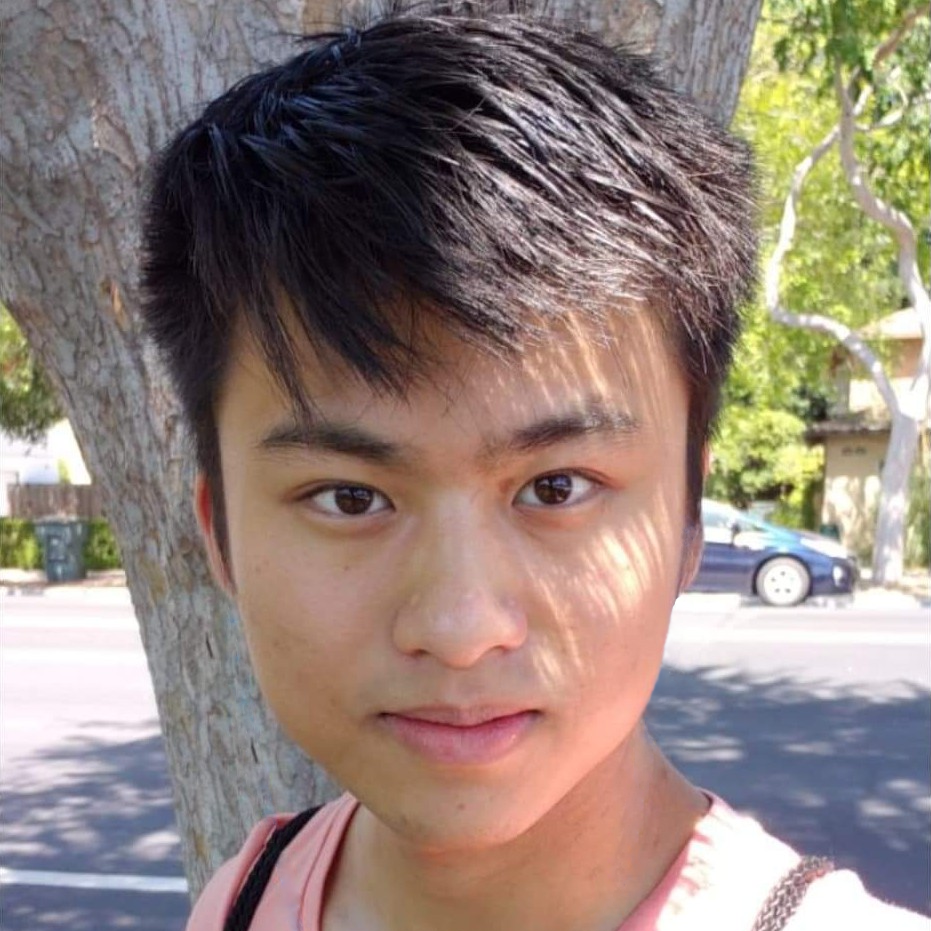
\includegraphics[height=2.3cm]{sam}
                %\caption*{The author, courtesy of Karl Winsor}
            \end{wrapfigure}
    %\let\thefootnote\relax\footnotetext{
        \normalsize
        Sam Tenka is a grad student in computer science 
        at MIT.  Their email address is
        \texttt{
            c{\tiny\ }%
            o{\tiny\ }%
            l{\tiny\ }%
            i{\tiny@}%
            m{\tiny\ }%
            i{\tiny\ }%
            t{\tiny\ }%
            .{\tiny\ }%
            e{\tiny\ }%
            d{\tiny\ }%
            u%
        }.
    %}
            %When not thinking about machines that learn, Sam can often be found
            %pretending to be a cow.  Sam enjoys memory over experience, pet
            %snails over pet spinach, left adjoints over right adjoints, and
            %analogies over lists.
\end{document}


